\begin{tikzpicture}[scale=0.75]
\tikzstyle{every node}=[font=\sffamily\small, inner sep=3pt, align=center]
\tikzstyle{every pin}=[align=center,fill=white]
\tikzstyle{dbnlabel}=[font=\sffamily\normalsize]
         
% Deformation field
        
\node[dbnlabel, rotate=90] at (-1.5,2.25) {Morphology DBN};
        
\begin{scope}[xshift=-20pt,yslant=0.63,xscale=0.4]

\node[transform shape,pin={[pin
distance=8]125:Displacement\\
field $u$}] (field) at (2,2)
{\includegraphics[width=4cm]{figures/deformation2.png}};

% \node[pin={[pin distance=0.6,overlay]93:Displacement\\
% field $u$}] at ($(field.north west)!0.1!(field.north east)$) {};

\end{scope}
         
% 3-channel input

\foreach \x in {0, 10, 20} {
\begin{scope}[xshift=\x pt]
%\ifnum\x=0
%\path
%\else
\draw[fill=white, fill opacity=0.75]
%\fi
  (0,0) coordinate(A\x) -- ++(90:4) coordinate (B\x) -- ++(30:2) coordinate
  (C\x) -- ++(-90:4) -- cycle;
  

% \begin{scope}[xshift=-50pt,yslant=0.63,xscale=0.4]  
% \node[transform shape,inner sep=0pt] at (2,2)
%   {\includegraphics[width=4cm]{deformation2.png}};
% \end{scope}
  
\draw (0,3)
   ++(30:0.25) \ifnum\x=20 coordinate (a1) \else -- +(0:10pt) +(0:0) \fi
-- ++(90:0.5)  \ifnum\x=20 coordinate (b1) \else -- +(0:10pt) +(0:0) \fi
-- ++(30:0.25) \ifnum\x=20 coordinate (c1) \else -- +(0:10pt) +(0:0) \fi
-- ++(-90:0.5) \ifnum\x=20 coordinate (d1) \else -- +(0:10pt) +(0:0) \fi
-- ++(210:0.25);
\end{scope}
}

%\node[below=4pt,xshift=-3pt] at (A0)  {$u_x$};
%\node[below=4pt] at (A10) {$u_y$};
%\node[below=4pt,xshift=3pt] at (A20) {$u_z$};

\node[pin={[pin distance=5pt]260:$u_x$}] at (A0)  {};
\node[pin={[pin distance=5pt]270:$u_y$}] at (A10)  {};
\node[pin={[pin distance=5pt]290:$u_z$}] at (A20)  {};

% Transition

\draw ($(a1)!0.5!(c1)$) ++(55pt,-5pt) coordinate (e1);
\draw (a1) -- (e1);
\draw (b1) -- (e1);
\draw (c1) --node[pin={[pin distance=1cm]40:Strided\\ convolution}] {} (e1);
\draw (d1) -- (e1);

% First layer hidden units

\foreach \x in {80,85,90,95,100,105} {
\begin{scope}[xshift=\x pt,yshift=1.5cm,scale=0.5]
\draw[fill=white, fill opacity=0.75]
  (0,0) coordinate(A\x) -- ++(90:4) coordinate (B\x) -- ++(30:2) coordinate
  (C\x) -- ++(-90:4) coordinate(D\x) -- cycle;
   
\draw (0,2.5)
   ++(30:0.25) \ifnum\x=105 coordinate (a2) \else -- +(0:10pt) +(0:0) \fi
-- ++(90:1)    \ifnum\x=105 coordinate (b2) \else -- +(0:10pt) +(0:0) \fi
-- ++(30:0.5)  \ifnum\x=105 coordinate (c2) \else -- +(0:10pt) +(0:0) \fi
-- ++(-90:1)   \ifnum\x=105 coordinate (d2) \else -- +(0:10pt) +(0:0) \fi
-- ++(210:0.5);
\end{scope}
}

\draw[decorate,decoration={brace,raise=20pt}] (B0|-C0) --node[above=25pt]
{Strided convolutional RBM} (C105|-C0);

\draw[decorate,decoration={brace,raise=4pt,mirror}]
%(A80) --node[below=8pt] {$N = 32$} (A80-|D105);
(A80) --node[below=8pt] {$N = 32$} (A80-|D105);

\draw ($(a2)!0.5!(c2)$) ++(0:38pt) coordinate (e2);
\draw (a2) -- (e2);
\draw (b2) -- (e2);
\draw (c2) -- (e2);
\draw (d2) -- (e2);

% Second layer hidden units

\foreach \x in {145, 150, ..., 175, 180} {
\begin{scope}[xshift=\x pt,yshift=2.25cm,scale=0.25]
\draw[fill=white, fill opacity=0.75]
  (0,0) coordinate(A\x) -- ++(90:4) coordinate (B\x) -- ++(30:2) coordinate
  (C\x) -- ++(-90:4) coordinate(D\x) -- cycle;
\draw (0,1.75)
   ++(30:0.25) \ifnum\x=180 coordinate (a3) \else -- +(0:20pt) +(0:0) \fi
-- ++(90:2)    \ifnum\x=180 coordinate (b3) \else -- +(0:20pt) +(0:0) \fi
-- ++(30:1)    \ifnum\x=180 coordinate (c3) \else -- +(0:20pt) +(0:0) \fi
-- ++(-90:2)   \ifnum\x=180 coordinate (d3) \else -- +(0:20pt) +(0:0) \fi
-- ++(210:1);
\end{scope}
}

\draw[decorate,decoration={brace,raise=4pt,mirror}]
(A145) --node[below=8pt] {$N = 64$} (A145-|D180);

\draw ($(a3)!0.5!(c3)$) ++(0:18pt) coordinate (e3);
\draw (a3) -- (e3);
\draw (b3) -- (e3);
\draw (c3) -- (e3);
\draw (d3) -- (e3);

% Third layer hidden units

\foreach \x in {200, 205, ..., 240} {
\begin{scope}[xshift=\x pt,yshift=2.625cm,scale=0.125]
\draw[fill=white, fill opacity=0.75]
  (0,0) coordinate(A\x) -- ++(90:4) coordinate (B\x) -- ++(30:2) coordinate
  (C\x) -- ++(-90:4) coordinate(D\x) -- cycle;
\end{scope}
}

% Forth layer visible units (dense)

\begin{scope}[xshift=280pt, yshift=2.75cm]
\foreach \x/\y in {0/-2, 1/-1.5, 2/-1, 3/-0.5, 4/0, 5/0.5, 6/1, 7/1.5, 8/2} {
  \node[circle, draw] (v\x) at (0,\y) {};
}
\end{scope}

\draw[shorten >=10pt,shorten <=10pt,dashed] (A240)--(v0.south west);
\draw[shorten >=10pt,shorten <=10pt,dashed] (A240|-C240)--
node[label=120:Vectorize\\ hidden units] {} (v8.north west);

\draw[decorate,decoration={brace,raise=4pt,mirror}]
(A200) --node[below=8pt,fill=white] {$N = 32$} (A200-|D240);

%\node[rotate=90,fill=white,align=center] at(270pt,2.75cm) {Serialize\\ hidden
%units};

% Forth layer hidden units (dense)

\begin{scope}[xshift=320pt, yshift=2.75cm]
\foreach \x/\y in {0/-1, 1/-0.5, 2/0, 3/0.5, 4/1} {
  \node[circle, draw] (h\x) at (0,\y) {};
}
\end{scope}

\foreach \x in {0, ..., 8} {
  \foreach \y in {0, ..., 4} {
    \draw[very thin] (v\x)--(h\y);
  }
}

\draw[decorate,decoration={brace,raise=20pt}] (v8.west|-C0)
--node[above=25pt] {Dense RBM} (h0.east|-C0);

% Fifth layer hidden units (distribution parameters)

\begin{scope}[xshift=360pt, yshift=2.75cm]
\foreach \x/\y in {1/0.25, 2/-0.25} {
  \node[circle, draw, label=0:$D_\x$] (D\x) at (0,\y) {};
}
\end{scope}

\foreach \x in {0, ..., 4} {
  \foreach \y in {1,2} {
    \draw[very thin] (h\x)--(D\y);
  }
}

% \draw[decorate,decoration={brace,raise=22pt}]
% (D1.north-|D1.east) --node[above,sloped] {Deformation\\ parameters}
% (D2.south-|D2.east);

%%%%%%%%%%%%%%%%%%%%%
% Lesion Model
%%%%%%%%%%%%%%%%%%%%%

\begin{scope}[yshift=-6cm]

\node[dbnlabel, rotate=90] at (-1.5,2.25) {Lesion DBN};

\begin{scope}[xshift=-25pt,yslant=0.63,xscale=0.4] 
\node[transform shape,pin={[pin distance=15]140:Lesion\\
mask $l$}] at (2,2)
  {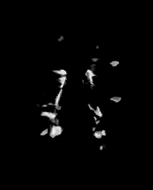
\includegraphics[height=4cm]{figures/lesions.png}};
\end{scope}

% 1-channel input

\foreach \x in {20} {
\begin{scope}[xshift=\x pt]
\draw[fill=white, fill opacity=0.75]
  (0,0) coordinate(A\x) -- ++(90:4) coordinate (B\x) -- ++(30:2) coordinate
  (C\x) -- ++(-90:4) coordinate (D\x) -- cycle;
  
\draw (0,3)
   ++(30:0.25) \ifnum\x=20 coordinate (a1) \else -- +(0:10pt) +(0:0) \fi
-- ++(90:0.5)  \ifnum\x=20 coordinate (b1) \else -- +(0:10pt) +(0:0) \fi
-- ++(30:0.25) \ifnum\x=20 coordinate (c1) \else -- +(0:10pt) +(0:0) \fi
-- ++(-90:0.5) \ifnum\x=20 coordinate (d1) \else -- +(0:10pt) +(0:0) \fi
-- ++(210:0.25);
\end{scope}
}

\node[pin=30:Visible\\ units] at ($(C20)!0.25!(D20)$) {};

% Transition

\draw ($(a1)!0.5!(c1)$) ++(55pt,-5pt) coordinate (e1);
\draw (a1) -- (e1);
\draw (b1) -- (e1);
\draw (c1) -- (e1);
\draw (d1) -- (e1);

% First layer hidden units

\foreach \x in {80,85,90,95,100,105} {
\begin{scope}[xshift=\x pt,yshift=1.5cm,scale=0.5]
\draw[fill=white, fill opacity=0.75]
  (0,0) coordinate(A\x) -- ++(90:4) coordinate (B\x) -- ++(30:2) coordinate
  (C\x) -- ++(-90:4) coordinate(D\x) -- cycle;
   
\draw (0,2.5)
   ++(30:0.25) \ifnum\x=105 coordinate (a2) \else -- +(0:10pt) +(0:0) \fi
-- ++(90:1)    \ifnum\x=105 coordinate (b2) \else -- +(0:10pt) +(0:0) \fi
-- ++(30:0.5)  \ifnum\x=105 coordinate (c2) \else -- +(0:10pt) +(0:0) \fi
-- ++(-90:1)   \ifnum\x=105 coordinate (d2) \else -- +(0:10pt) +(0:0) \fi
-- ++(210:0.5);
\end{scope}
}

\draw[decorate,decoration={brace,raise=4pt,mirror}]
%(A80) --node[below=8pt] {$N = 32$} (A80-|D105);
(A80) --node[below=8pt] {$N = 32$} (A80-|D105);

\draw ($(a2)!0.5!(c2)$) ++(0:38pt) coordinate (e2);
\draw (a2) -- (e2);
\draw (b2) -- (e2);
\draw (c2) -- (e2);
\draw (d2) -- (e2);

\node[pin=30:Hidden\\ units] at ($(C105)!0.2!(D105)$) {};

% Second layer hidden units

\foreach \x in {145, 150, ..., 175, 180} {
\begin{scope}[xshift=\x pt,yshift=2.25cm,scale=0.25]
\draw[fill=white, fill opacity=0.75]
  (0,0) coordinate(A\x) -- ++(90:4) coordinate (B\x) -- ++(30:2) coordinate
  (C\x) -- ++(-90:4) coordinate(D\x) -- cycle;
\draw (0,1.75)
   ++(30:0.25) \ifnum\x=180 coordinate (a3) \else -- +(0:20pt) +(0:0) \fi
-- ++(90:2)    \ifnum\x=180 coordinate (b3) \else -- +(0:20pt) +(0:0) \fi
-- ++(30:1)    \ifnum\x=180 coordinate (c3) \else -- +(0:20pt) +(0:0) \fi
-- ++(-90:2)   \ifnum\x=180 coordinate (d3) \else -- +(0:20pt) +(0:0) \fi
-- ++(210:1);
\end{scope}
}

\draw[decorate,decoration={brace,raise=4pt,mirror}]
(A145) --node[below=8pt] {$N = 64$} (A145-|D180);

\draw ($(a3)!0.5!(c3)$) ++(0:18pt) coordinate (e3);
\draw (a3) -- (e3);
\draw (b3) -- (e3);
\draw (c3) -- (e3);
\draw (d3) -- (e3);

% Third layer hidden units

\foreach \x in {200, 205, ..., 240} {
\begin{scope}[xshift=\x pt,yshift=2.625cm,scale=0.125]
\draw[fill=white, fill opacity=0.75]
  (0,0) coordinate(A\x) -- ++(90:4) coordinate (B\x) -- ++(30:2) coordinate
  (C\x) -- ++(-90:4) coordinate(D\x) -- cycle;
\end{scope}
}

%\node[rotate=90] at(270pt,2.75cm) {Serialize hidden units};

% Forth layer visible units (dense)

\begin{scope}[xshift=280pt, yshift=2.75cm]
\foreach \x/\y in {0/-2, 1/-1.5, 2/-1, 3/-0.5, 4/0, 5/0.5, 6/1, 7/1.5, 8/2} {
  \node[circle, draw] (V\x) at (0,\y) {};
}
\end{scope}

\draw[shorten >=10pt,shorten <=10pt,dashed] (A240)--(V0.south west);
\draw[shorten >=10pt,shorten <=10pt,dashed] (A240|-C240)--
%node[label=120:Vectorize\\ hidden units] {}
(V8.north west);

\draw[decorate,decoration={brace,raise=4pt,mirror}]
(A200) --node[below=8pt,fill=white] {$N = 32$} (A200-|D240);

%\node[rotate=90,fill=white,align=center] at(270pt,2.75cm) {Serialize\\ hidden
%units};

% Forth layer hidden units (dense)

\begin{scope}[xshift=320pt, yshift=2.75cm]
\foreach \x/\y in {0/-1, 1/-0.5, 2/0, 3/0.5, 4/1} {
  \node[circle, draw] (H\x) at (0,\y) {};
}
\end{scope}

\foreach \x in {0, ..., 8} {
  \foreach \y in {0, ..., 4} {
    \draw[very thin] (V\x)--(H\y);
  }
}

% Fifth layer hidden units (distribution parameters)

\begin{scope}[xshift=360pt, yshift=2.75cm]
\foreach \x/\y in {1/0.25, 2/-0.25} {
  \node[circle, draw, label=0:$L_\x$] (L\x) at (0,\y) {};
}
\end{scope}

\foreach \x in {0, ..., 4} {
  \foreach \y in {1,2} {
    \draw[very thin] (H\x)--(L\y);
  }
}
\end{scope}

%%%%%%%%%%%%%%
% Joint layer
%%%%%%%%%%%%%%

% yshift = 2.75 - 6/2 = -0.25

\begin{scope}[xshift=380pt, yshift=-0.25cm]
\foreach \x/\y in {1/-0.75, 2/-0.25, 3/0.25, 4/0.75} {
  \node[circle, draw, label=0:$J_\x$] (J\x) at (0,\y)
  {}; }
\end{scope}

\foreach \x in {0, ..., 4} {
  \foreach \y in {1, ..., 4} {
    \draw[very thin] (h\x)--(J\y);
    \draw[very thin] (H\x)--(J\y);
  }
}

\node[yshift=-15pt, fill=white, inner sep=3pt] at (h0) {$N = 16$};

\draw[decorate,decoration={brace,raise=30pt,mirror}] (V0.south-|J1)
--node[dbnlabel, below=35pt, sloped] {Joint DBN} (v8.north-|J1);

\end{tikzpicture}